\documentclass[a4paper,11pt]{article}
\usepackage[utf8]{inputenc}
\usepackage[english]{babel}
\usepackage{hyperref}
\usepackage{comment}
\usepackage{tikz}
\usetikzlibrary{arrows.meta, calc, positioning, shapes.geometric}
\usepackage[backend=biber, style=ieee]{biblatex}
\addbibresource{bib/references.bib}

\begin{document}

\selectlanguage{english}
\title{Verifiable Data Transformations in IoT Environments using Recursive zk-SNARKs}
\author{Ramón Felipe Kühne \\ Student number: 456119}
\date{}
\maketitle

\begin{center}
{\small
\textbf{Examiners}\\
First Examiner: Prof. Dr.-Ing. Stefan Tai\\
Second Examiner: Axel Küpper (SNET) or Stefan Schmid (INET)\\[1em]

\textbf{Supervisors}\\
Karl Christoph Wolf, Fabian Piper\\[1em]

Department of Information Systems Engineering (ISE), TU Berlin
}
\end{center}


\section*{Introduction}
Internet of Things (IoT) deployments such as smart home sensors, industrial monitors, and environmental sensing networks produce continuous high-resolution time-series data \cite{SmartMeterPrivacySurvey2023}. Aggregating this data in periodic batches—for example by summation or averaging—reduces communication and storage demands on resource-constrained devices but does not provide formal guarantees that the published aggregates correctly reflect all raw readings or that individual measurements remain confidential \cite{AStudyOnPrivacyPreserving2021}. In practice, simple aggregation schemes have been shown to leak sensitive patterns: Müller demonstrated that even hourly load profiles in smart homes can reveal user behavior \cite{muellerGewinnungVerhaltensprofilenAm2010}, and such schemes remain vulnerable to tampering or data omission without verifiable proofs \cite{bohliPrivacyModelSmart2010aa}.

Consider a typical smart home equipped with devices such as thermostats, motion sensors, smart meters, and voice assistants. These devices continuously collect detailed sensor readings, which, when aggregated over a defined interval, can reveal intimate insights into the occupants’ daily routines and personal habits \cite{chenSurveyZeroKnowledgeAuthentication2023}. For example, consistent energy consumption patterns reported by a smart meter over a given interval can indicate when residents are at home, asleep, or away, posing significant privacy risks \cite{molinaMarkhamEmbeddedSensingSystemsEnergyEfficiency2010, SmartMeterPrivacySurvey2023}. The problem is not that the physical meter is unreliable, but that the intermediary step (Local Aggregator) is a black box whose internal rules the user cannot control. Because the aggregation algorithm remains a black box, simple batch aggregation fails to ensure integrity and privacy simultaneously. Users generally trust individual measurement devices—such as a certified power meter—because they can directly observe the meter readout and verify its calibration. However, once these raw readings are collected by a local data aggregator and forwarded to an external electricity provider or cloud platform, the occupant loses visibility into which measurements were used or whether any values were omitted or altered \cite{kursawePrivacyFriendlyAggregationSmartGrid2011, rialPrivacypreservingSmartMetering2011}. This creates a trust gap: the resident sees each raw reading displayed in real time on the meter itself, but cannot confirm that the local data aggregator correctly summed all readings to produce the reported aggregate over the selected interval. Because the aggregation algorithm and data filtering steps remain non-transparent, there is a risk that data aggregators or cloud services could drop peak readings or adjust values to underreport usage, and the occupant has no mechanism to detect such manipulation. Economic incentives further exacerbate this issue: an electricity provider might underreport consumption to avoid peak-demand charges or penalties, since altering raw meter values at the device itself would be immediately noticed, but tampering during aggregation could go undetected \cite{elgoharyEvaluatingDemandCharges2023}. Consequently, users lack any effective way to verify that the published aggregate equals the sum of all raw measurements, making simple batch aggregation insufficient for both integrity and privacy.

Zero-Knowledge Proofs (ZKPs) can bridge this trust gap by allowing devices to cryptographically prove that aggregated data falls within expected parameters without revealing individual sensor readings \cite{swalensZkStreamFrameworkTrustworthy2024}. By generating succinct proofs of correct aggregation, ZKPs ensure that neither the local data aggregator nor the external electricity provider can manipulate or misreport data, while still hiding raw measurements \cite{swalensZkStreamFrameworkTrustworthy2024}. In this way, ZKPs drastically reduce the risk of data leaks by limiting the exposure of sensitive information and protect against data manipulation, since generating valid proofs for falsified data is computationally infeasible for attackers \cite{chenSurveyZeroKnowledgeAuthentication2023}. However, implementing ZKPs in IoT environments is technically challenging due to resource constraints: many cryptographic operations associated with ZKPs are computationally expensive. zkSNARKs address these limitations effectively by generating compact proofs and requiring constant-time verification independent of the computation complexity \cite{sallerasZPiEZeroknowledgeProofs2021}, making them ideal for scenarios where edge devices must regularly send proofs to a local data aggregator or an external electricity provider. Alternatives such as interactive protocols or zkSTARKs have significant drawbacks, including larger proofs, higher verification costs, or increased communication overhead \cite{berentsenWalkthroughSimpleZkSTARK2022a, sunSurveyZeroKnowledgeProof2021}.

Recursive zkSNARKs are particularly suited for continuous IoT data processing. Traditional methods would either generate separate proofs for every interval—leading to inefficiencies in managing numerous proofs—or create impractically large single proofs. Recursive composition elegantly addresses this by continuously combining smaller individual proofs into a single, compact end-proof \cite{zcashWhatAreZkSnarks2023}. For example, a resource-constrained device can periodically generate incremental proofs, chaining them together to ensure ongoing integrity verification; techniques like Nova demonstrate substantial performance advantages by efficiently aggregating multiple data verifications into a concise final proof \cite{kothapalli_nova_2022}. Recursive zkSNARKs thus provide scalable, resource-efficient verification suitable for IoT devices handling continuous data streams.

To fill this gap, we propose a general recursive zkSNARK-based architecture for privacy-preserving batch aggregation in IoT environments. Our design guarantees integrity by cryptographically binding each batch proof to all prior summaries so that any missing or altered reading invalidates the chain, confidentiality by revealing only the succinct recursive proof and hiding raw sensor values, and resource efficiency by optimizing circuits and proof composition for low-power IoT hardware. We implement and evaluate our prototype in a smart-home setting where edge devices collect measurements at fixed intervals and periodically submit aggregate proofs. The smart-home scenario offers a readily accessible and representative environment for development and testing, ensuring realistic data patterns and deployment conditions. This modular, application-independent framework can be readily adapted to industrial telemetry, environmental monitoring, and other continuous-streaming scenarios.

\subsection*{System Architecture}
\begin{center}
\vspace*{-0.2cm}
\hspace*{-0.5cm}
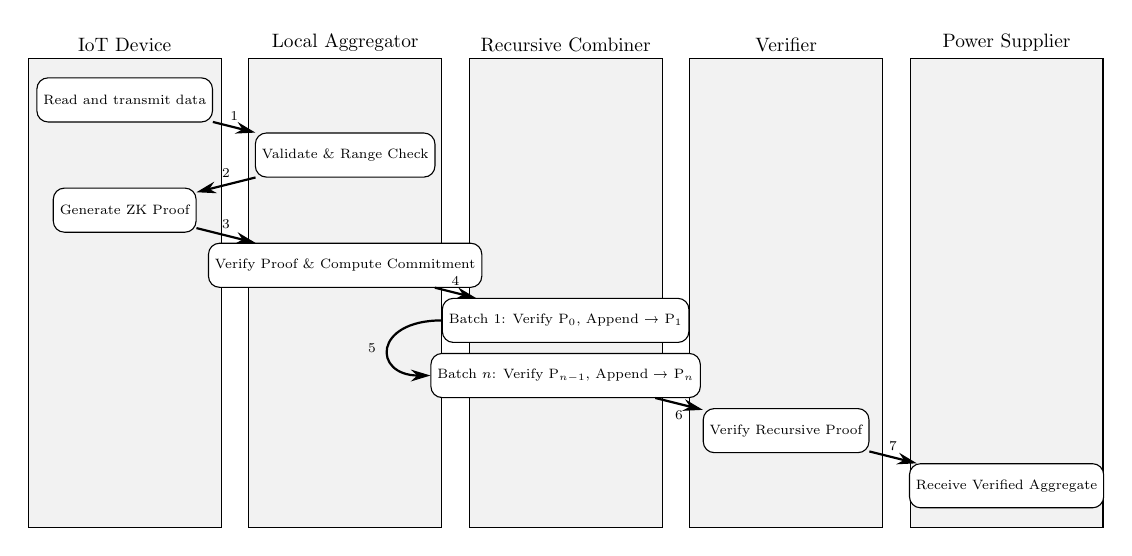
\begin{tikzpicture}[
    scale=0.7,                   % skaliert das gesamte Diagramm
    transform shape,             % skaliert auch Knoteninhalte
    lane/.style={draw, fill=gray!10, minimum width=3.5cm, minimum height=8.5cm},
    task/.style={draw, fill=white, rounded corners, minimum width=2.5cm, minimum height=0.8cm, font=\scriptsize},
    arrow/.style={-{Stealth[length=2.5mm,width=1.5mm]}, thick}
  ]

  % Swimlane-Rechtecke (vertikal an x=0,4,8,12,16)
  \node[lane]   (lane1) at (0,0)   {};
  \node[above] at (lane1.north)    {IoT Device};

  \node[lane]   (lane2) at (4,0)   {};
  \node[above] at (lane2.north)    {Local Aggregator};

  \node[lane]   (lane3) at (8,0)   {};
  \node[above] at (lane3.north)    {Recursive Combiner};

  \node[lane]   (lane4) at (12,0)  {};
  \node[above] at (lane4.north)    {Verifier};

  \node[lane]   (lane5) at (16,0)  {};
  \node[above] at (lane5.north)    {Power Supplier};

  \node[task]   (task1) at (0,3.5)        {Read and transmit data};
  \node[task]   (task2) at (4,2.5)        {Validate \& Range Check};
  \node[task]   (task3) at (0,1.5)        {Generate ZK Proof};
  \node[task]   (task4) at (4,0.5)        {Verify Proof \& Compute Commitment};
  \node[task] (task5_1) at (8,-0.5)       {Batch 1: Verify P$_0$, Append → P$_1$};
  \node[task] (task5_2) at (8,-1.5)       {Batch $n$: Verify P$_{n-1}$, Append → P$_n$};
  \node[task]   (task6) at (12,-2.5)      {Verify Recursive Proof};
  \node[task]   (task7) at (16,-3.5)      {Receive Verified Aggregate};

  \draw[arrow] (task1) -- node[above,font=\scriptsize] {1} (task2);
  \draw[arrow] (task2) -- node[above,font=\scriptsize] {2} (task3);
  \draw[arrow] (task3) -- node[above,font=\scriptsize] {3} (task4);
  \draw[arrow] (task4) -- node[above,font=\scriptsize] {4} (task5_1);
  \draw[arrow] (task5_1) .. controls (4.5,-0.5) and (4.5,-1.5) .. node[left,xshift=-0.1cm,font=\scriptsize] {5} (task5_2);
  \draw[arrow] (task5_2) -- node[below,font=\scriptsize] {6} (task6);
  \draw[arrow] (task6) -- node[above,font=\scriptsize] {7} (task7);

\end{tikzpicture}
\end{center}

Our architecture includes five distinct participants, as illustrated in the diagram above. \textit{IoT Devices} continuously collect fine‐grained sensor readings over a predefined time interval and transmit each raw measurement to the \textit{Local Aggregator}. The \textit{Local Aggregator} validates that the received measurement lies within predefined bounds; once validation succeeds, the IoT Device generates a zkSNARK proof \cite{sallerasZPiEZeroknowledgeProofs2021} that its interval summary (for example, total energy consumed) correctly reflects all private readings and satisfies the agreed constraints. The \textit{Local Aggregator} then verifies this proof and computes a short commitment encoding the validated batch summary, which it forwards to the next stage. The \textit{Recursive Combiner} verifies each incoming commitment against the previous recursive proof and integrates the new commitment into an updated recursive proof, ensuring that every batch remains cryptographically linked to all prior summaries \cite{zcashWhatAreZkSnarks2023,boweRecursiveProofComposition2019,dengZkTreeZeroKnowledgeRecursion2023}. Finally, the \textit{Verifier} checks the complete recursive proof in constant time \cite{kothapalli_nova_2022}. Because this proof remains succinct, verification can be executed with minimal overhead. The \textit{Power Supplier} then receives verified aggregate meaning it obtains only the compact, publicly verifiable proof (not any raw readings) and can trust that the published aggregate truly reflects every device’s data over all intervals. By cryptographically binding each batch summary to its entire history, any attempt to drop or alter a reading anywhere in the pipeline will break verification, thus ensuring end‐to‐end data integrity and preserving user privacy.

\subsection*{Applicability to Blockchain Contexts}
Although our primary focus is on IoT environments where a local aggregator or a centralized verifier checks proofs, this recursive zkSNARK architecture can be adapted to blockchain deployments with minimal changes. In a blockchain scenario, the public ledger takes on the role of the Verifier. Instead of sending aggregate proofs to a central backend, each edge device or a designated aggregator node submits its succinct recursive proof as a transaction on the chain. A smart contract running on that chain then executes the same zkSNARK verification steps, confirming that each batch summary correctly incorporates all prior intervals without revealing any raw sensor readings. Because zkSNARK proofs remain constant in size, the on‐chain gas costs stay fixed regardless of the number of intervals or devices involved. As a result, IoT devices can rely on the blockchain’s immutability and consensus rules for both data integrity and ordering. This means that the privacy‐preserving and integrity‐ensuring properties we designed for centralized settings carry over directly to fully decentralized architectures.

\section*{Related Work}
Existing work on privacy-preserving aggregation in IoT environments spans from early models in smart metering to more recent zkSNARK-based systems. Initial approaches used centralized aggregators or differential privacy mechanisms to mask individual device readings, yet these lacked formal integrity guarantees and remained vulnerable to statistical inference \cite{bohliPrivacyModelSmart2010aa, muellerGewinnungVerhaltensprofilenAm2010}. More advanced protocols, such as the secret-sharing scheme by Kursawe et al. \cite{kursawePrivacyFriendlyAggregationSmartGrid2011} and the on-device verification model by Rial and Danezis \cite{rialPrivacypreservingSmartMetering2011}, introduced stronger privacy controls, but still required interactive proofs for each batch and were not well suited for large-scale or autonomous IoT deployments. Blockchain-based architectures like ZGridBC demonstrated how zkSNARKs could ensure privacy and integrity in energy data markets, though they relied heavily on fixed-size batch commitments and incurred high on-chain costs \cite{miyamaeZGridBCZeroKnowledgeProof2021}. Meanwhile, off-chain solutions such as the netting protocols by Eberhardt et al. leveraged zkSNARKs via the ZoKrates toolkit to reduce settlement overhead, but generated a separate proof for every aggregation interval and did not support recursive composition \cite{eberhardtPrivacyPreservingNettingLocal2020, eberhardtZoKratesScalablePrivacyPreserving2018}.

Zero-Knowledge Succinct Non-Interactive Arguments of Knowledge (zkSNARKs) are cryptographic proof systems that allow a prover to demonstrate the validity of a statement without revealing any underlying information. The term \emph{succinct} indicates that these proofs are extremely compact, typically requiring minimal computational resources for verification, often just milliseconds. \emph{Non-interactive} means the proof is provided in a single message, eliminating the need for multiple rounds of communication between prover and verifier \cite{ZKSnarksEntmystifizierenSNARKs, schillerWasIstZkSNARKs2018}. Originally popularized through applications in blockchain technologies like Zcash \cite{zcashWhatAreZkSnarks2023}, zkSNARKs enable transactions and computations to be verified cryptographically without exposing sensitive details, making them highly suitable for privacy-sensitive IoT scenarios.

Recursive SNARKs, as introduced by Bitansky et al. in the form of proof-carrying data \cite{bitanskyRecursiveCompositionBootstrapping2012}, and later extended by Bowe et al. in the Halo framework \cite{boweRecursiveProofComposition2019}, offer constant-size recursive verification but have been primarily applied to static or blockchain data contexts. Deng and Du’s zkTree system similarly enables on-chain verification of hierarchically composed proofs but is tailored to ledger consistency \cite{dengZkTreeZeroKnowledgeRecursion2023}. The GENES architecture optimizes recursive proofs for throughput and memory in blockchain use cases, but makes assumptions that are incompatible with dynamic sensor data streams \cite{samudralaPerformanceAnalysisZeroKnowledge2024}. Finally, recent embedded zkSNARK applications such as zRA and ZEKRA extend zero-knowledge techniques to firmware and control-flow attestation \cite{ebrahimiInteractionIndependenceZkSNARKs2024, debesZEKRAZeroKnowledgeControlFlow2023}, yet operate on static codebases and lack mechanisms for continuous batch processing of input data.

While these systems demonstrate important building blocks, none of them provide a reusable, streaming-compatible zkSNARKs-based architecture specifically designed for resource-constrained IoT scenarios. In contrast, this thesis proposes a general framework that combines recursive proof composition, efficient circuit logic, and modular ZoKrates implementation to support unbounded IoT data aggregation with minimal overhead. The approach is distinct in that it avoids blockchain dependencies, supports ongoing recursive updates, and prioritizes adaptability across diverse IoT domains.

\begin{comment}
Circuit:
    /* range_check.zok */
// Verify each reading lies within [0, MAX]

import "hashes/sha256" as sha256;

// Max allowed value, e.g., 10000 (10 kWh per interval)
const u32 MAX = 10000;

// Range-check a single reading
def range_check(field value) -> bool {
    // value >= 0 is implicit for unsigned field
    if value > MAX {
        return false;
    }
    return true;
}

// Batch range-check for N readings
// Public output: merkle root of valid-flag list

def main(private field[N] readings) -> (field) {
    field[N] flags;
    for u32 i in 0..N {
        flags[i] = range_check(readings[i]) ? 1 : 0;
    }
    // Compute Merkle root of flags array
    field root = sha256.tree_root(flags);
    return root;
}


/* batch_aggregate.zok */
// Compute sum and optional average

def main(private field[N] readings) -> (field sum, field agg_commit) {
    field acc = 0;
    for u32 i in 0..N {
        acc = acc + readings[i];
    }
    // Pedersen commitment or simple hash commitment
    field[2] input = [acc, field(N)];
    field commitment = sha256.hash(input);
    return acc, commitment;
}


/* recursive_wrapper.zok */
// Verify previous proof and new batch together

import "proofs/verify" as verify;

// Public inputs: prev_commitment, prev_proof_hash, new_commitment

def main(field prev_commitment, field prev_proof_hash, field new_commitment,
         field[N] readings) -> (field combined_commitment) {
    // Verify the previous proof
    bool ok = verify(prev_proof_hash, [prev_commitment]);
    assert(ok == true);

    // Recompute new batch commitment
    field acc = 0;
    for u32 i in 0..N {
        acc = acc + readings[i];
    }
    field[2] input = [acc, field(N)];
    field batch_commit = sha256.hash(input);
    assert(batch_commit == new_commitment);

    // Combine previous and new commitments into one accumulator
    field[3] concat = [prev_commitment, new_commitment, prev_proof_hash];
    field combined = sha256.hash(concat);
    return combined;
}
\end{comment}
\section*{Research Question}
In this thesis, we propose a recursive zkSNARKs-based architecture specifically designed for privacy-preserving batch processing of streaming IoT data. The following research question will be addressed:

\medskip\noindent\textbf{How can a recursive zkSNARKs-based architecture be designed to ensure the confidentiality and integrity of batched IoT data streams while remaining efficient and practical for resource-constrained devices?}

\section*{Contributions}
This thesis makes the following contributions:

\begin{itemize}
  \item \textbf{Systematic design of a recursive zkSNARKs-based architecture} for privacy-preserving aggregation of time-series IoT data, developed from a comprehensive analysis of existing proof systems and their limitations in dynamic, streaming environments.
  
  \item \textbf{Implementation of a modular prototype in a smart-home environment} using the ZoKrates framework that supports recursive proof generation over multiple time intervals, ensuring confidentiality and integrity without exposing raw sensor data.
  
  \item \textbf{Demonstration of generalizability} through an application-independent circuit design and a transferable workflow.
  
  \item \textbf{Evaluation of performance, privacy and scalability} using Docker-based deployments that emulate constrained devices, validating the architecture’s practical feasibility through quantitative benchmarks and security analysis.
\end{itemize}

\section*{Methodology}
The research proceeds in two primary phases. In the first phase, existing privacy-preserving aggregation schemes, recursive zkSNARK constructions, and relevant IoT constraints are systematically reviewed. Particular attention is paid to the limitations of current approaches—such as the lack of recursive proof chaining, reliance on rigid batch structures, or limited adaptability to real-world data streams. Based on this review, a generalized, application-independent system architecture will be developed. This architecture defines a modular proof composition process designed for continuous sensor data and optimized for use on devices with limited computational and memory resources.

In the second phase, this architecture will be implemented as a recursive zkSNARK-based proof system using the ZoKrates framework. A key feature is the recursive aggregation mechanism, which securely connects multiple data batches into a single, verifiable proof. This approach aims to reduce communication and verification overhead while ensuring that raw input data remains confidential. The underlying circuit design will implement core logic such as data aggregation, range validation, and recursive linkage between proof intervals. We will demonstrate the prototype in a smart-home environment—where edge devices generate minute-level sensor readings and periodically report aggregates—to illustrate practical feasibility. Although demonstrated through this representative IoT scenario, the design is intended to be transferable across domains, including industrial telemetry, environmental monitoring, or smart infrastructure.


\section*{Evaluation}
The evaluation of the proposed system will be carried out on several levels. To simulate realistic IoT environments, all components will be deployed using Docker containers that emulate resource-constrained edge devices. This setup allows for reproducible benchmarks while maintaining close alignment with typical embedded system constraints.

First, the system’s privacy-preserving properties will be evaluated through a comparison of data observability before and after aggregation, using methodology inspired by Müller’s analysis of behavioral inference from load profiles \cite{muellerGewinnungVerhaltensprofilenAm2010}.

Second, a performance evaluation will assess the feasibility of recursive zkSNARK usage in constrained settings. Metrics such as proof generation time, verification latency, memory consumption, and proof size will be recorded across different batch configurations. These measurements follow established practices in prior work on zero-knowledge proof performance, such as Samudrala et al. \cite{samudralaPerformanceAnalysisZeroKnowledge2024}.

Third, a security analysis will validate the system’s resistance to manipulation by ensuring that any single malformed or inconsistent input invalidates the recursive proof chain. This guarantees the integrity of the entire aggregation process and enforces tamper-resilience at every step.

Lastly, we assess real-world applicability by analyzing the system’s communication overhead, maintenance complexity, and scalability in representative IoT use cases. Although tested through one specific scenario, the architecture will be shown to generalize to broader classes of time-series aggregation problems.

\begin{comment}
    verbesserungen:
mehr richtung bewertung

perfekte lösung recursive snark? nicht trivial
eher als ergebnis der arbeit 
unter folgendensn bedingungen lohnt sicher der einsatz von recursive snark
nicht nur zk snark sondern auch andere zkp
muss sinn ergeben dass es privacy preserving ist

ab dieser menge lohnt sich der einsatz von recursive snark
in evaluation machen
verschiedene metriken testen
wann snark wann recursive snark

gesamte logic vom circuit
ansatz: generalisiertes set von function
filter von set
median
minimum maximum

privacy preserving auch
einschätzen wie privacy garantiert wird
was bringt der mehrwert von recursive snark im bereich privacy

system vorstellen an dem ich die funktionalität messe
use case möglichst sinnvoll formulieren
\end{comment}

\printbibliography

\end{document}


